\documentclass[12pt]{article}

\usepackage{amsmath, mathtools}
\usepackage{amsfonts}
\usepackage{amssymb}
\usepackage{graphicx}
\usepackage{colortbl}
\usepackage{xr}
\usepackage{hyperref}
\usepackage{longtable}
\usepackage{xfrac}
\usepackage{tabularx}
\usepackage{float}
\usepackage{siunitx}
\usepackage{booktabs}
\usepackage{caption}
\usepackage{pdflscape}
\usepackage{afterpage}
\usepackage{verbatim}
\usepackage[round]{natbib}
\usepackage{colortbl}
\usepackage{hyperref}
\usepackage{lingmacros}
\usepackage{tree-dvips}
\usepackage{multirow}
\usepackage{blindtext}
\usepackage{colortbl}%For FR tables
\usepackage{hyperref}%For advanced hyperlinks
\usepackage{enumitem}%For advanced lists
\usepackage{pdfpages}
\usepackage{array}
\usepackage{tikz}
\usepackage{ulem}
\usetikzlibrary{shapes, arrows, positioning}

%\usepackage{refcheck}

\hypersetup{
    bookmarks=true,         % show bookmarks bar?
      colorlinks=true,       % false: boxed links; true: colored links
    linkcolor=red,          % color of internal links (change box color with linkbordercolor)
    citecolor=green,        % color of links to bibliography
    filecolor=magenta,      % color of file links
    urlcolor=cyan           % color of external links
}

%% Comments

\usepackage{color}

\newif\ifcomments\commentstrue %displays comments
%\newif\ifcomments\commentsfalse %so that comments do not display

\ifcomments
\newcommand{\authornote}[3]{\textcolor{#1}{[#3 ---#2]}}
\newcommand{\todo}[1]{\textcolor{red}{[TODO: #1]}}
\else
\newcommand{\authornote}[3]{}
\newcommand{\todo}[1]{}
\fi

\newcommand{\wss}[1]{\authornote{blue}{SS}{#1}} 
\newcommand{\plt}[1]{\authornote{magenta}{TPLT}{#1}} %For explanation of the template
\newcommand{\an}[1]{\authornote{cyan}{Author}{#1}}

%% Common Parts

\newcommand{\progname}{ProgName} % PUT YOUR PROGRAM NAME HERE
\newcommand{\authname}{Team \#, Team Name
\\ Student 1 name
\\ Student 2 name
\\ Student 3 name
\\ Student 4 name} % AUTHOR NAMES                  

\usepackage{hyperref}
    \hypersetup{colorlinks=true, linkcolor=blue, citecolor=blue, filecolor=blue,
                urlcolor=blue, unicode=false}
    \urlstyle{same}
                                


% For easy change of table widths
\newcommand{\colZwidth}{1.0\textwidth}
\newcommand{\colAwidth}{0.13\textwidth}
\newcommand{\colBwidth}{0.82\textwidth}
\newcommand{\colCwidth}{0.1\textwidth}
\newcommand{\colDwidth}{0.05\textwidth}
\newcommand{\colEwidth}{0.8\textwidth}
\newcommand{\colFwidth}{0.17\textwidth}
\newcommand{\colGwidth}{0.5\textwidth}
\newcommand{\colHwidth}{0.28\textwidth}

% Used so that cross-references have a meaningful prefix
\newcounter{defnum} %Definition Number
\newcommand{\dthedefnum}{GD\thedefnum}
\newcommand{\dref}[1]{GD\ref{#1}}
\newcounter{datadefnum} %Datadefinition Number
\newcommand{\ddthedatadefnum}{DD\thedatadefnum}
\newcommand{\ddref}[1]{DD\ref{#1}}
\newcounter{theorynum} %Theory Number
\newcommand{\tthetheorynum}{T\thetheorynum}
\newcommand{\tref}[1]{T\ref{#1}}
\newcounter{tablenum} %Table Number
\newcommand{\tbthetablenum}{T\thetablenum}
\newcommand{\tbref}[1]{TB\ref{#1}}
\newcounter{assumpnum} %Assumption Number
\newcommand{\atheassumpnum}{P\theassumpnum}
\newcommand{\aref}[1]{A\ref{#1}}
\newcounter{goalnum} %Goal Number
\newcommand{\gthegoalnum}{P\thegoalnum}
\newcommand{\gsref}[1]{GS\ref{#1}}
\newcounter{instnum} %Instance Number
\newcommand{\itheinstnum}{IM\theinstnum}
\newcommand{\iref}[1]{IM\ref{#1}}
\newcounter{reqnum} %Requirement Number
\newcommand{\rthereqnum}{P\thereqnum}
\newcommand{\rref}[1]{R\ref{#1}}
\newcounter{nfrnum} %NFR Number
\newcommand{\rthenfrnum}{NFR\thenfrnum}
\newcommand{\nfrref}[1]{NFR\ref{#1}}
\newcounter{lcnum} %Likely change number
\newcommand{\lthelcnum}{LC\thelcnum}
\newcommand{\lcref}[1]{LC\ref{#1}}

\usepackage{fullpage}

\newcommand{\deftheory}[9][Not Applicable]
{
\newpage
\noindent \rule{\textwidth}{0.5mm}

\paragraph{RefName: } \textbf{#2} \phantomsection 
\label{#2}

\paragraph{Label:} #3

\noindent \rule{\textwidth}{0.5mm}

\paragraph{Equation:}

#4

\paragraph{Description:}

#5

\paragraph{Notes:}

#6

\paragraph{Source:}

#7

\paragraph{Ref.\ By:}

#8

\paragraph{Preconditions for \hyperref[#2]{#2}:}
\label{#2_precond}

#9

\paragraph{Derivation for \hyperref[#2]{#2}:}
\label{#2_deriv}

#1

\noindent \rule{\textwidth}{0.5mm}

}

\begin{document}

\title{Software Requirements Specification for \progname: Synesthesia Wear} 
\author{\authname}
\date{\today}
	
\maketitle

~\newpage

\pagenumbering{roman}

\tableofcontents

\pagebreak

\section*{Revision History}

\begin{tabularx}{\textwidth}{p{3cm}p{2cm}X}
\toprule {\bf Date} & {\bf Version} & {\bf Notes}\\
\midrule
October 2, 2022 & 1.0 & Added Section 1 - Project Drivers\\

October 3, 2022 & 1.1 & Added Section 2,3 - Functional and Non-Functional Requirements\\

October 4, 2022 & 1.2 & Added Section 4,5 - Monitor and Controlled Variables, Traceability  \\
October 5, 2022 & 1.3 & Added Section 6 -  Project Issues \\
October 6, 2022 & 1.4 & Added References -  Reflection Appendix \\
April 4, 2023 & 1.5 & Updated for feedback and consistency\\
\bottomrule
\end{tabularx}

\vspace{5mm}
\noindent
This document describes the requirements for Synthesia Wear.
The template for the Software Requirements Specification (SRS)
is a subset of the Volere template (Robertson and Robertson, 2012).
\pagenumbering{arabic}

\section{Project Drivers}

\subsection{The Purpose of the Project}
The purpose of this project is to create an inexpensive and non-intrusive \sout{hearing aid bracelet} \textcolor{red}{wearable device} 
that provides an alternate channel for sound recognition for our users in their 
surroundings. \sout{First of all} \textcolor{red}{With this in mind}, Synesthesia Wear's main goal is to be able to provide an 
improved \sout{quality of life} \textcolor{red}{auditory awareness} for our users by \sout{instilling within them a sense of comfort 
knowing that our bracelet can help alleviate} \textcolor{red}{alleviating} their hearing difficulties in many environments. 
For this project, there will be 3 main aspects that must be done for its overall completion. 
The first one is to be able to design and create a small and lightweight bracelet that 
is comfortable for our users to wear while encompassing all the hardware needed for 
overall functionality. Simultaneously, the second aspect is one where the bracelet's 
sound detection is able to reliably detect as many significant sounds in our users' daily 
lives as possible. Lastly, an app is going to be made so that it has a user-friendly user interface (UI) that is easy to use and will allow users to easily be able to configure their sound 
detection settings for their bracelets.

\subsection{The Stakeholders}

\subsubsection{The Client}
\textbf{N/A}

\subsubsection{The Customers}
The customers of this project would be people in the general public who would want or 
need an inexpensive and non-intrusive \sout{bracelet} \textcolor{red}{wearable device} that helps with their 
\sout{hearing} \textcolor{red}{awareness in their surroundings}. Furthermore, 
people who are in loud environments may want to purchase Synesthesia Wear as well since 
hearing is likely obstructed and sound recognition through touch/vibration would be very 
appealing.

\subsubsection{Other Stakeholders}
The Developers:
The developers of this project are the members of Strone. Our job is to develop a 
\sout{bracelet} \textcolor{red}{wearable device} that is capable of assisting in the sound recognition of users within their 
surroundings. Throughout this project's entirety, we will test and change/improve 
aspects that we may deem necessary.

\subsection{Constraints}

\subsubsection{Solution Constraints}
The Synesthesia Wear application should be able to run on many computers, laptops, and
phones. For phones, the application will be supported on IOS and Android OS. 
Furthermore, for laptops/computers, the application will be supported by macOS and Windows 
OS. With all this in mind, it is assumed that implementing for other mobile/laptop/computer 
OS's would be unprofitable and wasteful to maintain.   

\subsubsection{Implementation Environment of the Current System}
\begin{figure}[h]
  \centering
  \begin{tikzpicture}[node distance = 3cm]
  \tikzstyle{terminator} = [rectangle, draw, text centered, rounded corners, minimum height=2em]
  \tikzstyle{decision} = [diamond, draw, text centered, minimum height=2em]
  \tikzstyle{data}=[trapezium, draw, text centered, trapezium left angle=60, trapezium right angle=120, minimum height=2em]
  \tikzstyle{connector} = [draw, -latex']
  \node [terminator, fill=green!20] (start) {\textbf{Developers}};
  \node [data, fill=blue!20, right = 1.5cm of start] (app) {Application};
  \node [data, fill=blue!20, below of=app] (wearableDevice) {Wearable Device};
  \node [decision, fill=blue!20, right = 1.5cm of app] (mobileDevice) {Mobile Device};
  \node [terminator, fill=green!20, right = 1.5cm of mobileDevice] (user) {\textbf{User}};
  \path [connector] (start) -- (app);
  \path [connector] (start) |- (wearableDevice);
  \path [connector] (app) -- (wearableDevice); 
  \path [connector] (mobileDevice) -- (app);
  \path [connector] (user) -- (mobileDevice);
  \path [connector] (user) |- (wearableDevice);
  \end{tikzpicture}
  \caption{Implementation Environment}
\end{figure}

\subsubsection{Partner or Collaborative Applications}
Synesthesia Wear does not have any partner or collaborative applications. However, it 
does rely upon the fact that the user is using the application on a device that supports
IOS, Android, macOS, or Windows OS. 

\subsubsection{Anticipated Workplace Environment}
There is no specific anticipated workplace environment for this product. Ideally, this 
\sout{bracelet} \textcolor{red}{wearable device} and corresponding app can be used anywhere so long as they have a \textcolor{red}{mobile} device that 
supports IOS, Android, macOS, or Windows OS.

\subsubsection{Schedule Constraints}
It has been decided that this project is to be completed by the week of April 5th, 2022.
As a result, this project's scheduling will be executed over a timespan of a \sout{bit more 
than} \textcolor{red}{little over} 7 months.

\subsubsection{Budget Constraints}
For this project, the budget has been dictated to be no more than \$750 from the entirety 
of all group members. With this in mind, there is no issues with the application as all 
software tools and resources are expected to use open-source material found online. Thus, 
most/all of the budget will likely be spent towards designing and creating the lightweight, 
non-intrusive, and comfortable \sout{bracelet} \textcolor{red}{wearable device}.

\subsubsection{Enterprise Constraints}
The finished application will be available for anyone to use. However, the Synesthesia Wear 
\sout{bracelet} \textcolor{red}{wearable device} will need to be purchased as it costs money and time to buy all the components and 
build it. 

\subsection{Naming Conventions and Terminology}
\subsubsection{Definitions of All Terms, Including Acronyms, Used by Stakeholders Involved in the Project }
\begin{table} [H]
  \centering
  \arrayrulecolor{white}
  \begin{tabular}{|>{\centering\arraybackslash}p{7cm}|>{\centering\arraybackslash}p{8cm}} 
  \hline
  \rowcolor[rgb]{0.071,0.49,0.698} \textcolor{white}{ACRONYNM/ABBREVIATION} & \textcolor{white}{INTENDED MEANING}\\ 
  \hline
  \rowcolor[rgb]{0.675,0.827,0.902} SYWR & Synesthesia Wear\\ 
  \hline
  \rowcolor[rgb]{0.675,0.827,0.902} UI & User Interface\\ 
  \hline
  \rowcolor[rgb]{0.675,0.827,0.902} OS & Operating System\\ 
  \hline
  \rowcolor[rgb]{0.675,0.827,0.902} Etc & Et Cetera\\ 
  \hline
  \rowcolor[rgb]{0.675,0.827,0.902} Wi-Fi & Wireless Fidelity\\ 
  \hline
  \rowcolor[rgb]{0.675,0.827,0.902} IDE & Integrated Development Environment\\ 
  \hline
  \rowcolor[rgb]{0.675,0.827,0.902} GL & Gitlab\\ 
  \hline
  \rowcolor[rgb]{0.675,0.827,0.902} Product & The \sout{bracelet} \textcolor{red}{wearable device} and appliction being developed as a whole, in its finished state\\ 
  \hline
  \rowcolor[rgb]{0.675,0.827,0.902} Project & The development of the \sout{bracelet} \textcolor{red}{wearable device} and application\\ 
  \hline
  \rowcolor[rgb]{0.675,0.827,0.902} Customer & The person(s) that will use the finished product\\ 
  \hline
  \end{tabular}
  \label{Definitions}
  \caption{Definitions}
\end{table}

\subsection{Relevant Facts and Assumptions}

\subsubsection{Relevant Facts}
There are a few rules that the team must adhere to during the development of this
project. Firstly, each developer must attend the group meeting before the submission
of a deliverable to ensure that everyone has given their opinions and approval of the
work, sort out any discrepancies, correct errors, and then satisfactorily submit with
some time to spare. Furthermore, another rule that must be adhered is the fact that 
each developer has the right to question and ask for further explanations from others 
on their work. This is because both/all parties' work is related in some way or another 
and so the extra clarification and effort would be to all developers' benefit. 

\subsubsection{Assumptions}
The developers are assuming that all software resources that will be used in the 
creation of the project will be open source software that is free for us to use. 
Furthermore, it is assumed that the majority/all of our users will have access to 
a device that supports macOS, Windows OS, IOS, or Android OS.

\section{Functional Requirements}
\subsection{The Scope of the Work and the Product}
\subsubsection{Context Diagram}

\begin{figure}[H]
  \begin{center}
    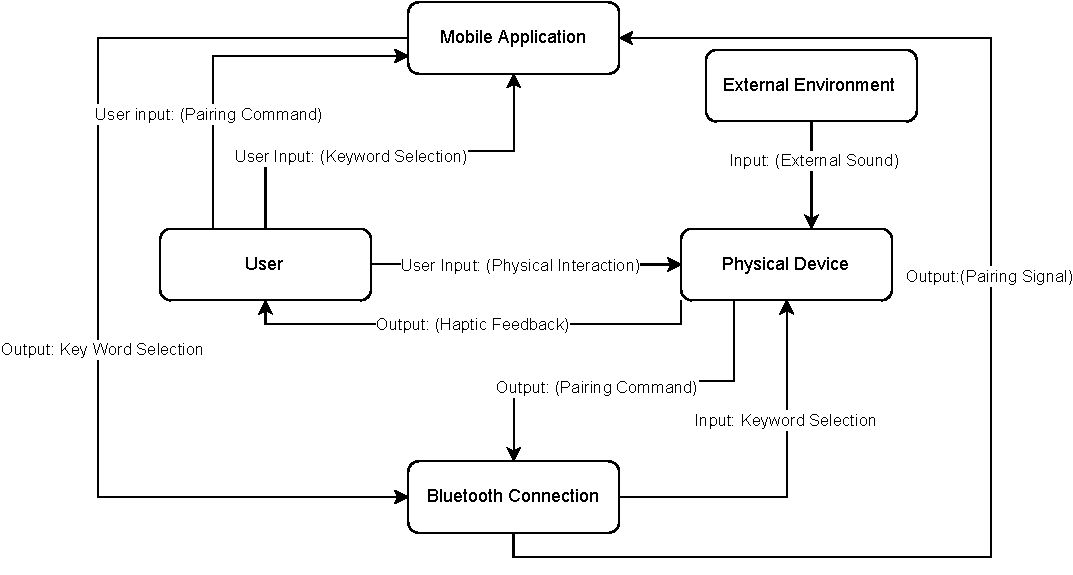
\includegraphics{WC.pdf}
  \caption{Context Diagram}
  \label{ContextDiagram} 
  \end{center}
\end{figure}

\subsubsection{Individual Product Use Cases}
\begin{figure}[H]
  \begin{center}
    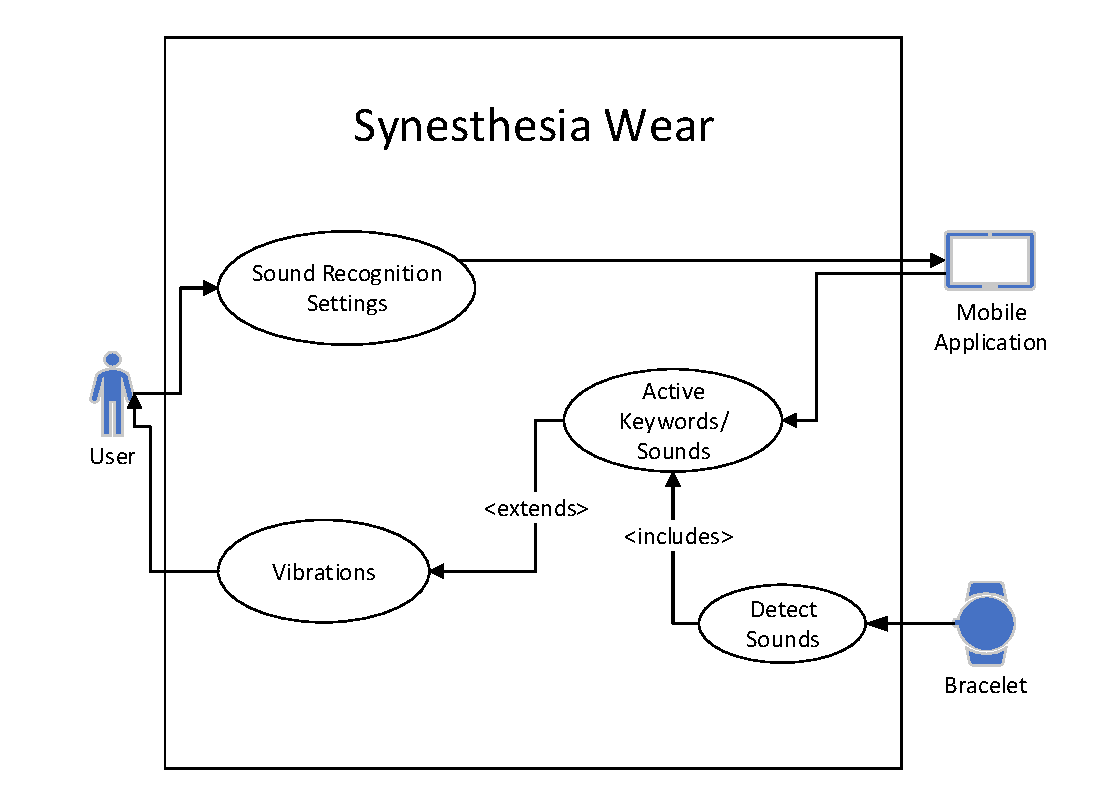
\includegraphics{UCD.pdf}
    \caption{User Case Diagram}
  \label{ContextDiagram} 
  \end{center}
\end{figure}

\subsection{Functional Requirements}
\newcounter{FR}
\setcounter{FR}{0}
%FR1
\stepcounter{FR}
\begin{table}[H]
  \centering
  \arrayrulecolor{white}
  \begin{tabular}{|p{3cm}|p{11cm}|} 
  \hline
  \rowcolor[rgb]{0.071,0.49,0.698} \textcolor{white}{Requirement No} & \textcolor{white}{FR-\arabic{FR}}                                           \\ 
  \hline
  \rowcolor[rgb]{0.675,0.827,0.902} Description                                            & The device is able to pick up sounds in the environment of the user.  \\ 
  \hline
  \rowcolor[rgb]{0.675,0.827,0.902} Fit Criterion                                              & The data received by the device shall match the sounds supplied \sout{to} \textcolor{red}{from} the device's surroundings .                       \\ 
  \hline
  \rowcolor[rgb]{0.675,0.827,0.902} Dependencies                                           & N/A                                                                   \\ 
  \hline
  \end{tabular}
  \label{FR-1}
  \arrayrulecolor{black}
\end{table}
%FR2
\stepcounter{FR}
\begin{table}[H]
  \centering
  \arrayrulecolor{white}
  \begin{tabular}{|p{3cm}|p{11cm}|} 
  \hline
  \rowcolor[rgb]{0.071,0.49,0.698} \textcolor{white}{Requirement No} & \textcolor{white}{FR-\arabic{FR}}                                             \\ 
  \hline
  \rowcolor[rgb]{0.675,0.827,0.902} Description                                            & The device has to be able to correctly classify different sounds \textcolor{red}{that the user has specified. These sounds are limited to any distinct audible sounds whose time does not exceed 1 second}.   \\ 
  \hline
  \rowcolor[rgb]{0.675,0.827,0.902} Fit Criterion                                              & \sout{Will compare} Test sounds and the device classifications \sout{shall} \textcolor{red}{should} match the \sout{true} \textcolor{red}{expected} classification of the sounds.                         \\ 
  \hline
  \rowcolor[rgb]{0.675,0.827,0.902} Dependencies                                           &  FR-1, FR-4                                                                   \\ 
  \hline
  \end{tabular}
  \arrayrulecolor{black}
\end{table}
%FR3
\stepcounter{FR}
\begin{table}[H]
  \centering
  \arrayrulecolor{white}
  \begin{tabular}{|p{3cm}|p{11cm}|} 
  \hline
  \rowcolor[rgb]{0.071,0.49,0.698} \textcolor{white}{Requirement No} & \textcolor{white}{FR-\arabic{FR}}                                             \\ 
  \hline
  \rowcolor[rgb]{0.675,0.827,0.902} Description                                            & \textcolor{red}{The device has to be able to classify unspecified sounds as random sounds.}   \\ 
  \hline
  \rowcolor[rgb]{0.675,0.827,0.902} Fit Criterion                                              & Random sounds should have the highest confidence for the random classification which will exist even if the user has not specified them        \\ 
  \hline
  \rowcolor[rgb]{0.675,0.827,0.902} Dependencies                                           &  FR-2, FR-4                                                                   \\ 
  \hline
  \end{tabular}
  \arrayrulecolor{black}
\end{table}
\begin{comment}
\begin{table}
  \centering
  \arrayrulecolor{white}
  \begin{tabular}{|p{3cm}|p{11cm}|} 
  \hline
  \rowcolor[rgb]{0.071,0.49,0.698} \textcolor{white}{Requirement No} & \textcolor{white}{FR-3}                                             \\ 
  \hline
  \rowcolor[rgb]{0.675,0.827,0.902} Description                                            & The device is able to receive data from an external device.  \\ 
  \hline
  \rowcolor[rgb]{0.675,0.827,0.902} Fit Criterion                                              & The received data shall agree with the sent data.                        \\ 
  \hline
  \rowcolor[rgb]{0.675,0.827,0.902} Dependencies                                           & N/A                                                                   \\ 
  \hline
  \end{tabular}
  \arrayrulecolor{black}
\end{table}
\end{comment}
%FR4
\stepcounter{FR}
\begin{table}[H]
  \centering
  \arrayrulecolor{white}
  \begin{tabular}{|p{3cm}|p{11cm}|} 
  \hline
  \rowcolor[rgb]{0.071,0.49,0.698} \textcolor{white}{Requirement No} & \textcolor{white}{FR-\arabic{FR}}                                             \\ 
  \hline
  \rowcolor[rgb]{0.675,0.827,0.902} Description                                            & The device has to be able to \textcolor{red}{store user defined classifications until any changes are made by the user}.  \\ 
  \hline
  \rowcolor[rgb]{0.675,0.827,0.902} Fit Criterion                                              & The device should be able to retain different user specified classifications until a user change command is asserted.                       \\ 
  \hline
  \rowcolor[rgb]{0.675,0.827,0.902} Dependencies                                           & FR-5                                                                 \\ 
  \hline
  \end{tabular}
  \arrayrulecolor{black}
\end{table}
%FR5
\stepcounter{FR}
\begin{table}[H]
  \centering
  \arrayrulecolor{white}
  \begin{tabular}{|p{3cm}|p{11cm}|} 
  \hline
  \rowcolor[rgb]{0.071,0.49,0.698} \textcolor{white}{Requirement No} & \textcolor{white}{FR-\arabic{FR}}                                             \\ 
  \hline
  \rowcolor[rgb]{0.675,0.827,0.902} Description                                            & The device has to be able to \textcolor{red}{communicate via Bluetooth in order to add, delete or modify} its classifications and their specifications.  \\ 
  \hline
  \rowcolor[rgb]{0.675,0.827,0.902} Fit Criterion                                              & The commands sent through Bluetooth shall make the intended changes in \sout{classification} \textcolor{red}{the active settings of the device}.                       \\ 
  \hline
  \rowcolor[rgb]{0.675,0.827,0.902} Dependencies                                           & FR-4                                                                  \\ 
  \hline
  \end{tabular}
  \arrayrulecolor{black}
\end{table}
%FR6
\stepcounter{FR}
\begin{table}[H]
  \centering
  \arrayrulecolor{white}
  \begin{tabular}{|p{3cm}|p{11cm}|} 
  \hline
  \rowcolor[rgb]{0.071,0.49,0.698} \textcolor{white}{Requirement No} & \textcolor{white}{FR-\arabic{FR}}                                             \\ 
  \hline
  \rowcolor[rgb]{0.675,0.827,0.902} Description                                            & The device is able to provide feedback to the user.  \\ 
  \hline
  \rowcolor[rgb]{0.675,0.827,0.902} Fit Criterion                                              & The feedback should alert the user that the device is trying to communicate some information.                       \\ 
  \hline
  \rowcolor[rgb]{0.675,0.827,0.902} Dependencies                                           & N/A                                                                   \\ 
  \hline
  \end{tabular}
  \arrayrulecolor{black}
\end{table}
%FR7
\stepcounter{FR}
\begin{table}[H]
  \centering
  \arrayrulecolor{white}
  \begin{tabular}{|p{3cm}|p{11cm}|} 
  \hline
  \rowcolor[rgb]{0.071,0.49,0.698} \textcolor{white}{Requirement No} & \textcolor{white}{FR-\arabic{FR}}                                             \\ 
  \hline
  \rowcolor[rgb]{0.675,0.827,0.902} Description                                            & The feedback provided is the appropriate feedback.  \\ 
  \hline
  \rowcolor[rgb]{0.675,0.827,0.902} Fit Criterion                                              & The feedback shall convey what signal classification was detected.                      \\ 
  \hline
  \rowcolor[rgb]{0.675,0.827,0.902} Dependencies                                           & FR-2, FR-4                                                                  \\ 
  \hline
  \end{tabular}
  \arrayrulecolor{black}
\end{table}
%FR8
\stepcounter{FR}
\begin{table}[H]
  \centering
  \arrayrulecolor{white}
  \begin{tabular}{|p{3cm}|p{11cm}|} 
  \hline
  \rowcolor[rgb]{0.071,0.49,0.698} \textcolor{white}{Requirement No} & \textcolor{white}{FR-\arabic{FR}}                                             \\ 
  \hline
  \rowcolor[rgb]{0.675,0.827,0.902} Description                                            & \textcolor{red}{The device will be able to process sounds of different intensities and noise levels.}  \\ 
  \hline
  \rowcolor[rgb]{0.675,0.827,0.902} Fit Criterion                                              & Able to do sound processing on different kinds of sounds.                      \\ 
  \hline
  \rowcolor[rgb]{0.675,0.827,0.902} Dependencies                                           & FR-1, FR-2                                                                  \\ 
  \hline
  \end{tabular}
  \arrayrulecolor{black}
\end{table}

\section{Non-Functional Requirements}
\newcounter{NFR}
\setcounter{NFR}{0}

\subsection{Look and Feel Requirements}

\subsubsection{Appearance Requirements}
%NFR-001
\stepcounter{NFR}
\begin{table}[H]
  \centering
  \arrayrulecolor{white}
  \begin{tabular}{|p{3cm}|p{11cm}|} 
  \hline
  \rowcolor[rgb]{0.071,0.49,0.698} \textcolor{white}{Requirement No} & \textcolor{white}{NFR-\arabic{NFR}}                                             \\ 
  \hline
  \rowcolor[rgb]{0.675,0.827,0.902} Description  & \begin{itemize}[leftmargin=*] 
    \item The UI of the application will contain a home page that displays the company logo and an option to pair the device.
    \item The UI of the application will have buttons which will have different colors for different functionalities.
    \item The UI will have a separate page for pairing the device and a page for configuring which voices you want to be alerted by. 
    \item The device will be a uniform material finish and contain an on button and Bluetooth pairing button. 
    \item The device will have a distinguished charging port built into the finished material.
  \end{itemize}  \\ 
  \hline
  \rowcolor[rgb]{0.675,0.827,0.902} Fit Criterion & Check that the UI and device satisfy mandated requirements.                      \\ 
  \hline
  \rowcolor[rgb]{0.675,0.827,0.902} Dependencies  & NFR-2                                                                \\ 
  \hline
  \end{tabular}
  \arrayrulecolor{black}
\end{table}

\subsubsection{Style Requirements}
%NFR-002
\stepcounter{NFR}
\begin{table}[H]
  \centering
  \arrayrulecolor{white}
  \begin{tabular}{|p{3cm}|p{11cm}|} 
  \hline
  \rowcolor[rgb]{0.071,0.49,0.698} \textcolor{white}{Requirement No} & \textcolor{white}{NFR-\arabic{NFR}}                                             \\ 
  \hline
  \rowcolor[rgb]{0.675,0.827,0.902} Description  & \begin{itemize}[leftmargin=*] 
    \item The UI will use consistent buttons, fonts, and color palette.
    \item The device will automatically begin the pairing process when button is pressed 
 \item Buttons on the UI should be easily identified. \sout{and responsive.}
 \end{itemize}  \\ 
  \hline
  \rowcolor[rgb]{0.675,0.827,0.902} Fit Criterion & Check that all buttons of the UI and the device correctly communicate back.
  \\ 
  \hline
  \rowcolor[rgb]{0.675,0.827,0.902} Dependencies  & NFR-1                                                                 \\ 
  \hline
  \end{tabular}
  \arrayrulecolor{black}
\end{table}

\subsection{Usability and Humanity Requirement}

\subsubsection{Ease of Use Requirements}
%NFR-003
\stepcounter{NFR}
\begin{table}[H]
  \centering
  \arrayrulecolor{white}
  \begin{tabular}{|p{3cm}|p{11cm}|} 
  \hline
  \rowcolor[rgb]{0.071,0.49,0.698} \textcolor{white}{Requirement No} & \textcolor{white}{NFR-\arabic{NFR}}                                             \\ 
  \hline
  \rowcolor[rgb]{0.675,0.827,0.902} Description  & \begin{itemize}[leftmargin=*] 
    \item The device shall be usable by any user with basic understanding of mobile applications and bluetooth devices. 
    \item The product should provide support that assists users in avoiding mistakes. 
    \end{itemize}  \\ 
  \hline
  \rowcolor[rgb]{0.675,0.827,0.902} Fit Criterion & 90\% of a sample group can go through the application without a manual.
  \\ 
  \hline
  \rowcolor[rgb]{0.675,0.827,0.902} Dependencies  & NFR-4, NFR-1                                                                  \\ 
  \hline
  \end{tabular}
  \arrayrulecolor{black}
\end{table}

\subsubsection{Personalization and Internationalization Requirements}
%NFR-004
\stepcounter{NFR}
\begin{table}[H]
  \centering
  \arrayrulecolor{white}
  \begin{tabular}{|p{3cm}|p{11cm}|} 
  \hline
  \rowcolor[rgb]{0.071,0.49,0.698} \textcolor{white}{Requirement No} & \textcolor{white}{NFR-\arabic{NFR}}                                             \\ 
  \hline
  \rowcolor[rgb]{0.675,0.827,0.902} Description  & \begin{itemize}[leftmargin=*] 
    \item Devices should allow users to pick and choose their desired sounds to be notified by.
    \item Application of the product should allow users to choose preferred language
    \item User Manual for the device will be written in primary language of each region device is sold
    \end{itemize}  \\ 
  \hline
  \rowcolor[rgb]{0.675,0.827,0.902} Fit Criterion & A sample group shall be able to change and manage their preferences.
  \\ 
  \hline
  \rowcolor[rgb]{0.675,0.827,0.902} Dependencies  & FR-5                                                                 \\ 
  \hline
  \end{tabular}
  \arrayrulecolor{black}
\end{table}
\subsubsection{Learning Requirements}
%NFR-005
\stepcounter{NFR}
\begin{table}[H]
  \centering
  \arrayrulecolor{white}
  \begin{tabular}{|p{3cm}|p{11cm}|} 
  \hline
  \rowcolor[rgb]{0.071,0.49,0.698} \textcolor{white}{Requirement No} & \textcolor{white}{NFR-\arabic{NFR}}                                             \\ 
  \hline
  \rowcolor[rgb]{0.675,0.827,0.902} Description  & This device and the corresponding application shall be able to be used by users with no prior training within 5 minutes.   \\ 
  \hline
  \rowcolor[rgb]{0.675,0.827,0.902} Fit Criterion & A sample group shall take less than 5 minutes to start using the product.
  \\ 
  \hline
  \rowcolor[rgb]{0.675,0.827,0.902} Dependencies  & NFR-3                                                                 \\ 
  \hline
  \end{tabular}
  \arrayrulecolor{black}
\end{table}
\subsubsection{Understandability and Politeness Requirements}
%NFR-006
\stepcounter{NFR}
\begin{table}[H]
  \centering
  \arrayrulecolor{white}
  \begin{tabular}{|p{3cm}|p{11cm}|} 
  \hline
  \rowcolor[rgb]{0.071,0.49,0.698} \textcolor{white}{Requirement No} & \textcolor{white}{NFR-\arabic{NFR}}                                             \\ 
  \hline
  \rowcolor[rgb]{0.675,0.827,0.902} Description  & The device and the application will use icons when the icon is commonly associated with a standard action such as a bluetooth logo for pairing.   \\ 
  \hline
  \rowcolor[rgb]{0.675,0.827,0.902} Fit Criterion & Check that the UI and device satisfy mandated requirements.
  \\ 
  \hline
  \rowcolor[rgb]{0.675,0.827,0.902} Dependencies  & NFR-1, NFR-2                                                                  \\ 
  \hline
  \end{tabular}
  \arrayrulecolor{black}
\end{table}
\subsubsection{Accessibility Requirements}
%NFR-007
\stepcounter{NFR}
\begin{table}[H]
  \centering
  \arrayrulecolor{white}
  \begin{tabular}{|p{3cm}|p{11cm}|} 
  \hline
  \rowcolor[rgb]{0.071,0.49,0.698} \textcolor{white}{Requirement No} & \textcolor{white}{NFR-\arabic{NFR}}                                             \\ 
  \hline
  \rowcolor[rgb]{0.675,0.827,0.902} Description  & Anybody who can operate a mobile device and is capable of wearing a ring/bracelet will be able to operate the device.    \\ 
  \hline
  \rowcolor[rgb]{0.675,0.827,0.902} Fit Criterion & Same fit criteria as NFR-3
  \\ 
  \hline
  \rowcolor[rgb]{0.675,0.827,0.902} Dependencies  & NFR-3                                                                  \\ 
  \hline
  \end{tabular}
  \arrayrulecolor{black}
\end{table}
\subsubsection{Convenience Requirements} 
%NFR-008
\stepcounter{NFR}
\begin{table}[H]
  \centering
  \arrayrulecolor{white}
  \begin{tabular}{|p{3cm}|p{11cm}|} 
  \hline
  \rowcolor[rgb]{0.071,0.49,0.698} \textcolor{white}{Requirement No} & \textcolor{white}{NFR-\arabic{NFR}}                                             \\ 
  \hline
  \rowcolor[rgb]{0.675,0.827,0.902} Description  & If the phone falls out of range, the device should automatically re-pair to a known device when the device is back in range.    \\ 
  \hline
  \rowcolor[rgb]{0.675,0.827,0.902} Fit Criterion & POC testing when a phone gets disconnected it should connect back when back in range.
  \\ 
  \hline
  \rowcolor[rgb]{0.675,0.827,0.902} Dependencies  & N/A                                                                  \\ 
  \hline
  \end{tabular}
  \arrayrulecolor{black}
\end{table}
\subsection{Performance Requirements}

\subsubsection{Speed and Latency Requirements} 
%NFR-009
\stepcounter{NFR}
\begin{table}[H]
  \centering
  \arrayrulecolor{white}
  \begin{tabular}{|p{3cm}|p{11cm}|} 
  \hline
  \rowcolor[rgb]{0.071,0.49,0.698} \textcolor{white}{Requirement No} & \textcolor{white}{NFR-\arabic{NFR}}                                             \\ 
  \hline
  \rowcolor[rgb]{0.675,0.827,0.902} Description  & \begin{itemize}[leftmargin=*] 
    \item The device shall process sound and react, with haptic feedback, if keywords are found in 1 second of response time
\item Interactions between the user and UI should have a response time of 1ms
\item First time pairing of the device should take no longer than 1 minute
\item Recurring connections of the device should take no longer than 10 seconds.  
\end{itemize}  \\ 
  \hline
  \rowcolor[rgb]{0.675,0.827,0.902} Fit Criterion & Check that the device satisfies the above requirements.
  \\ 
  \hline
  \rowcolor[rgb]{0.675,0.827,0.902} Dependencies  & FR-1, FR-2, FR-6, FR-7, NFR-3, NFR-8                                                                  \\ 
  \hline
  \end{tabular}
  \arrayrulecolor{black}
\end{table}

\subsubsection{Safety-Critical Requirements}   
%NFR-010
\stepcounter{NFR}
\begin{table}[H]
  \centering
  \arrayrulecolor{white}
  \begin{tabular}{|p{3cm}|p{11cm}|} 
  \hline
  \rowcolor[rgb]{0.071,0.49,0.698} \textcolor{white}{Requirement No} & \textcolor{white}{NFR-\arabic{NFR}}                                             \\ 
  \hline
  \rowcolor[rgb]{0.675,0.827,0.902} Description  & Battery of the device should be shielded to prevent any direct contact with the user.  \\ 
  \hline
  \rowcolor[rgb]{0.675,0.827,0.902} Fit Criterion & When the device is worn there is no way to directly touch the hardware components other than the buttons and ports. 
  \\ 
  \hline
  \rowcolor[rgb]{0.675,0.827,0.902} Dependencies  & N/A                                                                  \\ 
  \hline
  \end{tabular}
  \arrayrulecolor{black}
\end{table}

\subsubsection{Precision or Accuracy Requirements}
%NFR-011
\stepcounter{NFR}
\begin{table}[H]
  \centering
  \arrayrulecolor{white}
  \begin{tabular}{|p{3cm}|p{11cm}|} 
  \hline
  \rowcolor[rgb]{0.071,0.49,0.698} \textcolor{white}{Requirement No} & \textcolor{white}{NFR-\arabic{NFR}}                                             \\ 
  \hline
  \rowcolor[rgb]{0.675,0.827,0.902} Description  & Devices shall only miss-process noise or give a false haptic feedback once in every x amount of processes (Where x is determined by the team).   \\ 
  \hline
  \rowcolor[rgb]{0.675,0.827,0.902} Fit Criterion & Check that the device satisfies the above requirements.
  \\ 
  \hline
  \rowcolor[rgb]{0.675,0.827,0.902} Dependencies  & FR-2, FR-7, NFR-9                                                                  \\ 
  \hline
  \end{tabular}
  \arrayrulecolor{black}
\end{table}

\subsubsection{Reliability and Availability Requirements}
%NFR-012
\stepcounter{NFR}
\begin{table}[H]
  \centering
  \arrayrulecolor{white}
  \begin{tabular}{|p{3cm}|p{11cm}|} 
  \hline
  \rowcolor[rgb]{0.071,0.49,0.698} \textcolor{white}{Requirement No} & \textcolor{white}{NFR-\arabic{NFR}}                                             \\ 
  \hline
  \rowcolor[rgb]{0.675,0.827,0.902} Description  & \begin{itemize}[leftmargin=*] 
    \item Battery life of the device should last for 12 hours of use.
\item Sound sensor should be listening for keywords at all times while the device is powered on.
\item \sout{Application should have an uptime of 24 hours a day, 365 days a year.}
\end{itemize}  \\ 
  \hline
  \rowcolor[rgb]{0.675,0.827,0.902} Fit Criterion & Check that the device satisfies the above requirements.
  \\ 
  \hline
  \rowcolor[rgb]{0.675,0.827,0.902} Dependencies  & FR-1, NFR-9                                                                 \\ 
  \hline
  \end{tabular}
  \arrayrulecolor{black}
\end{table}

\subsubsection{Robustness or Fault-Tolerance Requirements} 
%NFR-013
\stepcounter{NFR}
\begin{table}[H]
  \centering
  \arrayrulecolor{white}
  \begin{tabular}{|p{3cm}|p{11cm}|} 
  \hline
  \rowcolor[rgb]{0.071,0.49,0.698} \textcolor{white}{Requirement No} & \textcolor{white}{NFR-\arabic{NFR}}                                             \\ 
  \hline
  \rowcolor[rgb]{0.675,0.827,0.902} Description  & \begin{itemize}[leftmargin=*] 
   \item  Device should be able to filter out noise in loud environments while still picking up on keywords.
    \item Device should still function even if the bluetooth gets disconnected from the user's mobile device.
    \end{itemize}  \\ 
  \hline
  \rowcolor[rgb]{0.675,0.827,0.902} Fit Criterion & Testing of accuracy in different environments
  \\ 
  \hline
  \rowcolor[rgb]{0.675,0.827,0.902} Dependencies  & FR-1, NFR-11                                                                   \\ 
  \hline
  \end{tabular}
  \arrayrulecolor{black}
\end{table}

\subsubsection{Capacity Requirements}  
%NFR-014
\stepcounter{NFR}
\begin{table}[H]
  \centering
  \arrayrulecolor{white}
  \begin{tabular}{|p{3cm}|p{11cm}|} 
  \hline
  \rowcolor[rgb]{0.071,0.49,0.698} \textcolor{white}{Requirement No} & \textcolor{white}{NFR-\arabic{NFR}}                                             \\ 
  \hline
  \rowcolor[rgb]{0.675,0.827,0.902} Description  & \begin{itemize}[leftmargin=*] 
    \item System should only record the 5 keywords as chosen by the user of the device.
    \item Application should record the inputted keywords by the user even if the application is closed.
    \end{itemize}  \\ 
  \hline
  \rowcolor[rgb]{0.675,0.827,0.902} Fit Criterion & Check that the device satisfies the above requirement.
  \\ 
  \hline
  \rowcolor[rgb]{0.675,0.827,0.902} Dependencies  & NFR-9                                                                  \\ 
  \hline
  \end{tabular}
  \arrayrulecolor{black}
\end{table}

\subsubsection{ Scalability or Extensibility Requirements } 
%NFR-015
\stepcounter{NFR}
\begin{table}[H]
  \centering
  \arrayrulecolor{white}
  \begin{tabular}{|p{3cm}|p{11cm}|} 
  \hline
  \rowcolor[rgb]{0.071,0.49,0.698} \textcolor{white}{Requirement No} & \textcolor{white}{NFR-\arabic{NFR}}                                             \\ 
  \hline
  \rowcolor[rgb]{0.675,0.827,0.902} Description  & The device should be capable of processing the current 5 keywords and upwards of 5 additional keywords two years after launch.   \\ 
  \hline
  \rowcolor[rgb]{0.675,0.827,0.902} Fit Criterion & NFR-14 shall be achieved along with scope that more words can be added. 
  \\ 
  \hline
  \rowcolor[rgb]{0.675,0.827,0.902} Dependencies  & NFR-14                                                                  \\ 
  \hline
  \end{tabular}
  \arrayrulecolor{black}
\end{table}

\subsubsection{ Longevity Requirements } 
%NFR-016
\stepcounter{NFR}
\begin{table}[H]
  \centering
  \arrayrulecolor{white}
  \begin{tabular}{|p{3cm}|p{11cm}|} 
  \hline
  \rowcolor[rgb]{0.071,0.49,0.698} \textcolor{white}{Requirement No} & \textcolor{white}{NFR-\arabic{NFR}}                                             \\ 
  \hline
  \rowcolor[rgb]{0.675,0.827,0.902} Description  & The device should have an expected lifetime of 5 years considering regular maintenance and use cases.   \\ 
  \hline
  \rowcolor[rgb]{0.675,0.827,0.902} Fit Criterion & The estimated battery lifecycle shall be above 5 years.
  \\ 
  \hline
  \rowcolor[rgb]{0.675,0.827,0.902} Dependencies  & NFR-12                                                                  \\ 
  \hline
  \end{tabular}
  \arrayrulecolor{black}
\end{table}

\subsection{Operational and Environmental Requirements} 

\subsubsection{Expected Physical Environment} 
%NFR-017
\stepcounter{NFR}
\begin{table}[H]
  \centering
  \arrayrulecolor{white}
  \begin{tabular}{|p{3cm}|p{11cm}|} 
  \hline
  \rowcolor[rgb]{0.071,0.49,0.698} \textcolor{white}{Requirement No} & \textcolor{white}{NFR-\arabic{NFR}}                                             \\ 
  \hline
  \rowcolor[rgb]{0.675,0.827,0.902} Description  & \begin{itemize}[leftmargin=*] 
    \item The device will be used by individuals in normal day to day activities.
    \item The product dimensions should allow fitment on either wrist or finger of the user. 
    \item The application shall run on any mobile device that is using an IOS or Android operating system. 
    \end{itemize}  \\ 
  \hline
  \rowcolor[rgb]{0.675,0.827,0.902} Fit Criterion & Using a study group check that the device operates during normal day activities, fits on all users, and runs on their desired phones. 
  \\ 
  \hline
  \rowcolor[rgb]{0.675,0.827,0.902} Dependencies  & NFR-12, NFR-13, NFR-1, NFR-2                                                                 \\ 
  \hline
  \end{tabular}
  \arrayrulecolor{black}
\end{table}

\subsubsection{ Requirements for Interfacing with Adjacent Systems} 
%NFR-018
\stepcounter{NFR}
\begin{table}[H]
  \centering
  \arrayrulecolor{white}
  \begin{tabular}{|p{3cm}|p{11cm}|} 
  \hline
  \rowcolor[rgb]{0.071,0.49,0.698} \textcolor{white}{Requirement No} & \textcolor{white}{NFR-\arabic{NFR}}                                             \\ 
  \hline
  \rowcolor[rgb]{0.675,0.827,0.902} Description  & The device will be able to interface with an application running on the user's mobile device.
  \\ 
  \hline
  \rowcolor[rgb]{0.675,0.827,0.902} Fit Criterion & Check that the device correctly pairs and reacts with updates from the application.
  \\ 
  \hline
  \rowcolor[rgb]{0.675,0.827,0.902} Dependencies  & NFR-8, NFR-14, NFR-15                                                                  \\ 
  \hline
  \end{tabular}
  \arrayrulecolor{black}
\end{table}

\subsubsection{Productization Requirements} 
\textbf{N/A}
\subsubsection{Release Requirements} 
%NFR-019
\stepcounter{NFR}
\begin{table}[H]
  \centering
  \arrayrulecolor{white}
  \begin{tabular}{|p{3cm}|p{11cm}|} 
  \hline
  \rowcolor[rgb]{0.071,0.49,0.698} \textcolor{white}{Requirement No} & \textcolor{white}{NFR-\arabic{NFR}}                                             \\ 
  \hline
  \rowcolor[rgb]{0.675,0.827,0.902} Description  & Yearly software releases will be deployed to improve the signal processing of the device as well as to maintain the corresponding application of the device.\\ 
  \hline
  \rowcolor[rgb]{0.675,0.827,0.902} Fit Criterion & Ensure software updates have been deployed on a year to year basis.
  \\ 
  \hline
  \rowcolor[rgb]{0.675,0.827,0.902} Dependencies  & N/A                                                                  \\ 
  \hline
  \end{tabular}
  \arrayrulecolor{black}
\end{table}

\subsection{Maintainability and Support Requirements}

\subsubsection{Maintenance Requirements}  
%NFR-020
\stepcounter{NFR}
\begin{table}[H]
  \centering
  \arrayrulecolor{white}
  \begin{tabular}{|p{3cm}|p{11cm}|} 
  \hline
  \rowcolor[rgb]{0.071,0.49,0.698} \textcolor{white}{Requirement No} & \textcolor{white}{NFR-\arabic{NFR}}                                             \\ 
  \hline
  \rowcolor[rgb]{0.675,0.827,0.902} Description  & Updates to the software of the device should only require the application to be down for one day at a time.  \\ 
  \hline
  \rowcolor[rgb]{0.675,0.827,0.902} Fit Criterion & If an update is pushed, check to ensure application down time does not exceed 24 hours.
  \\ 
  \hline
  \rowcolor[rgb]{0.675,0.827,0.902} Dependencies  & N/A                                                                  \\ 
  \hline
  \end{tabular}
  \arrayrulecolor{black}
\end{table}

\subsubsection{Supportability Requirements } 
\textbf{N/A}

\subsubsection{Adaptability Requirements}  
%NFR-021
\stepcounter{NFR}
\begin{table}[H]
  \centering
  \arrayrulecolor{white}
  \begin{tabular}{|p{3cm}|p{11cm}|} 
  \hline
  \rowcolor[rgb]{0.071,0.49,0.698} \textcolor{white}{Requirement No} & \textcolor{white}{NFR-\arabic{NFR}}                                             \\ 
  \hline
  \rowcolor[rgb]{0.675,0.827,0.902} Description  & Product is expected to interface with Android and IOS mobile devices.   \\ 
  \hline
  \rowcolor[rgb]{0.675,0.827,0.902} Fit Criterion & Using mobile devices running Android and IOS attempt to pair the device.
  \\ 
  \hline
  \rowcolor[rgb]{0.675,0.827,0.902} Dependencies  & NFR-18                                                                 \\ 
  \hline
  \end{tabular}
  \arrayrulecolor{black}
\end{table}

\subsection{Security Requirements }

\subsubsection{Access Requirements }  
%NFR-022
\stepcounter{NFR}
\begin{table}[H]
  \centering
  \arrayrulecolor{white}
  \begin{tabular}{|p{3cm}|p{11cm}|} 
  \hline
  \rowcolor[rgb]{0.071,0.49,0.698} \textcolor{white}{Requirement No} & \textcolor{white}{NFR-\arabic{NFR}}                                             \\ 
  \hline
  \rowcolor[rgb]{0.675,0.827,0.902} Description  & \begin{itemize}[leftmargin=*] 
    \item Nobody will have access to the signals being processed. Sounds should be processed and deleted in real time.
    \item Any user will have access to the UI of the application but only developers will have access to the backend of the code. 
    \end{itemize}  \\ 
  \hline
  \rowcolor[rgb]{0.675,0.827,0.902} Fit Criterion & Check that nobody has access to signals after processing is complete and ensure anybody has access to the UI.

  \\ 
  \hline
  \rowcolor[rgb]{0.675,0.827,0.902} Dependencies  & N/A                                                                  \\ 
  \hline
  \end{tabular}
  \arrayrulecolor{black}
\end{table}

\subsubsection{Integrity Requirements }  
%NFR-023
\stepcounter{NFR}
\begin{table}[H]
  \centering
  \arrayrulecolor{white}
  \begin{tabular}{|p{3cm}|p{11cm}|} 
  \hline
  \rowcolor[rgb]{0.071,0.49,0.698} \textcolor{white}{Requirement No} & \textcolor{white}{NFR-\arabic{NFR}}                                             \\ 
  \hline
  \rowcolor[rgb]{0.675,0.827,0.902} Description  & The device will filter out redundant \textcolor{red}{high frequency} external noise in order to improve the integrity of our signal processing.  \\ 
  \hline
  \rowcolor[rgb]{0.675,0.827,0.902} Fit Criterion & \textcolor{red}{Reduce amplitude by 90\% for all frequencies higher than 1/4 of sampling frequency (16kHz). }
  \\ 
  \hline
  \rowcolor[rgb]{0.675,0.827,0.902} Dependencies  & FR-1, FR-2, NFR-13, NFR-15                                                                  \\ 
  \hline
  \end{tabular}
  \arrayrulecolor{black}
\end{table}

\subsubsection{Privacy Requirements }  
%NFR-024
\stepcounter{NFR}
\begin{table}[H]
  \centering
  \arrayrulecolor{white}
  \begin{tabular}{|p{3cm}|p{11cm}|} 
  \hline
  \rowcolor[rgb]{0.071,0.49,0.698} \textcolor{white}{Requirement No} & \textcolor{white}{NFR-\arabic{NFR}}                                             \\ 
  \hline
  \rowcolor[rgb]{0.675,0.827,0.902} Description  & The product will protect the users right to privacy by not keeping a record of the data it takes in for the signal processing.  \\ 
  \hline
  \rowcolor[rgb]{0.675,0.827,0.902} Fit Criterion & N/A
  \\ 
  \hline
  \rowcolor[rgb]{0.675,0.827,0.902} Dependencies  & NFR-22                                                                  \\ 
  \hline
  \end{tabular}
  \arrayrulecolor{black}
\end{table}

\subsubsection{Audit Requirements }  
\textbf{N/A}
\subsubsection{Immunity Requirements}  
\textbf{N/A}
\subsection{Cultural Requirements }

\subsubsection{Cultural Requirements} 
%NFR-025
\stepcounter{NFR}
\begin{table}[H]
  \centering
  \arrayrulecolor{white}
  \begin{tabular}{|p{3cm}|p{11cm}|} 
  \hline
  \rowcolor[rgb]{0.071,0.49,0.698} \textcolor{white}{Requirement No} & \textcolor{white}{NFR-\arabic{NFR}}                                             \\ 
  \hline
  \rowcolor[rgb]{0.675,0.827,0.902} Description  & \begin{itemize}[leftmargin=*] 
    \item \sout{The product will only support English at launch but will strive to include more languages based on regions of purchase.}
    \item The application and the device will both have zero references pertaining to religions, ethinic groups or any cultures. 
    \end{itemize}  \\ 
  \hline
  \rowcolor[rgb]{0.675,0.827,0.902} Fit Criterion & Check that all buttons of the UI and the device correctly communicate back.
  \\ 
  \hline
  \rowcolor[rgb]{0.675,0.827,0.902} Dependencies  & FR-2, FR-4                                                                  \\ 
  \hline
  \end{tabular}
  \arrayrulecolor{black}
\end{table}

\subsection{Legal Requirements}

\subsubsection{Legal Compliance Requirements } 
%NFR-026
\stepcounter{NFR}
\begin{table}[H]
  \centering
  \arrayrulecolor{white}
  \begin{tabular}{|p{3cm}|p{11cm}|} 
  \hline
  \rowcolor[rgb]{0.071,0.49,0.698} \textcolor{white}{Requirement No} & \textcolor{white}{NFR-\arabic{NFR}}                                             \\ 
  \hline
  \rowcolor[rgb]{0.675,0.827,0.902} Description  & The product will comply with all laws and regulations pertaining to regions where it is sold and distributed.  \\ 
  \hline
  \rowcolor[rgb]{0.675,0.827,0.902} Fit Criterion & Take a law professional's opinion that the product follows all laws and regulations.
  \\ 
  \hline
  \rowcolor[rgb]{0.675,0.827,0.902} Dependencies  & N/A                                                                  \\ 
  \hline
  \end{tabular}
  \arrayrulecolor{black}
\end{table}

\subsubsection{Standards Compliance Requirements}  
%NFR-027
\stepcounter{NFR}
\begin{table}[H]
  \centering
  \arrayrulecolor{white}
  \begin{tabular}{|p{3cm}|p{11cm}|} 
  \hline
  \rowcolor[rgb]{0.071,0.49,0.698} \textcolor{white}{Requirement No} & \textcolor{white}{NFR-\arabic{NFR}}                                             \\ 
  \hline
  \rowcolor[rgb]{0.675,0.827,0.902} Description  & Product will adhere to any Open License agreements.  \\ 
  \hline
  \rowcolor[rgb]{0.675,0.827,0.902} Fit Criterion & Consult the license agreement to ensure no breach of license. 
  \\ 
  \hline
  \rowcolor[rgb]{0.675,0.827,0.902} Dependencies  & N/A                                                                  \\ 
  \hline
  \end{tabular}
  \arrayrulecolor{black}
\end{table}

\subsection{Health and Safety Requirements}
%NFR-028
\stepcounter{NFR}
\begin{table}[H]
  \centering
  \arrayrulecolor{white}
  \begin{tabular}{|p{3cm}|p{11cm}|} 
  \hline
  \rowcolor[rgb]{0.071,0.49,0.698} \textcolor{white}{Requirement No} & \textcolor{white}{NFR-\arabic{NFR}}                                             \\ 
  \hline
  \rowcolor[rgb]{0.675,0.827,0.902} Description  & \begin{itemize}[leftmargin=*] 
    \item Product will use certified batteries.
    \item Product will use haptic feedback that is not intrusive to the user.
    \end{itemize}  \\ 
  \hline
  \rowcolor[rgb]{0.675,0.827,0.902} Fit Criterion & Check haptic feedback on a group study of people and ensure all batteries have been certified.
  \\ 
  \hline
  \rowcolor[rgb]{0.675,0.827,0.902} Dependencies  & NFR-26                                                                  \\ 
  \hline
  \end{tabular}
  \arrayrulecolor{black}
\end{table}

\section{Monitor and Control Variables}

\center

\begin{tabular}{|p{3cm}|p{4.5cm}|p{4.5cm}|p{3cm}| }
 \hline
 \multicolumn{4}{|c|}{Variables} \\
 \hline
 Monitored& Description & Controlled & Description\\
 \hline
 Pairing Command  &  Start the pairing process  & Key Word Selection & Sound selection  \\
 \hline
External Sound &  Monitor the incoming sounds & Haptic Feedback & Motor signals \\
\hline
User Selection & If device is active & Mode Selection & What mode is required \\
\hline


\end{tabular}
\captionof{table}{Monitor and Control Variables}

\raggedright

\section{Traceability}
 	
\subsection{Traceability Diagram}

\begin{figure}[H]
  \begin{center}
    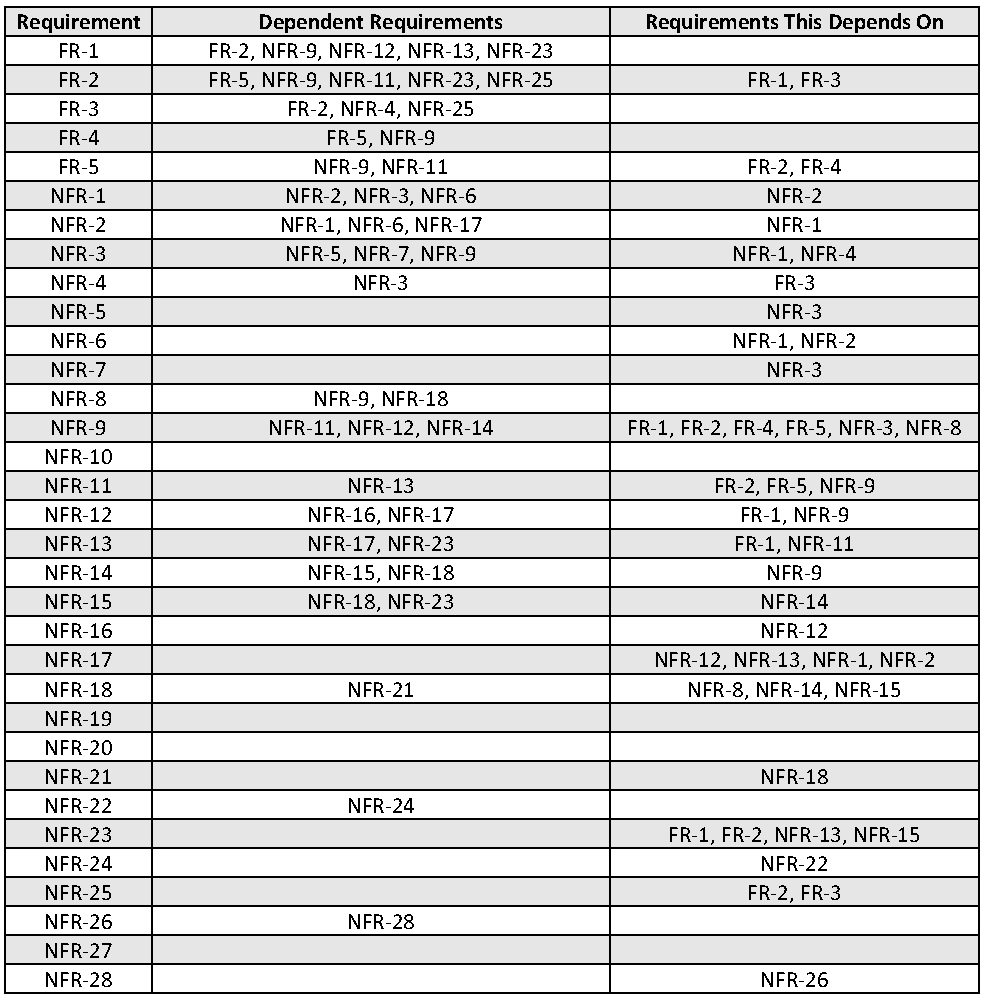
\includegraphics{T-Matrix.pdf}
  \caption{Traceability Diagram}
  \label{TraceDiagram} 
  \end{center}
\end{figure}

\subsection{Phase in Diagram}

\begin{figure}[H]
  \begin{center}
    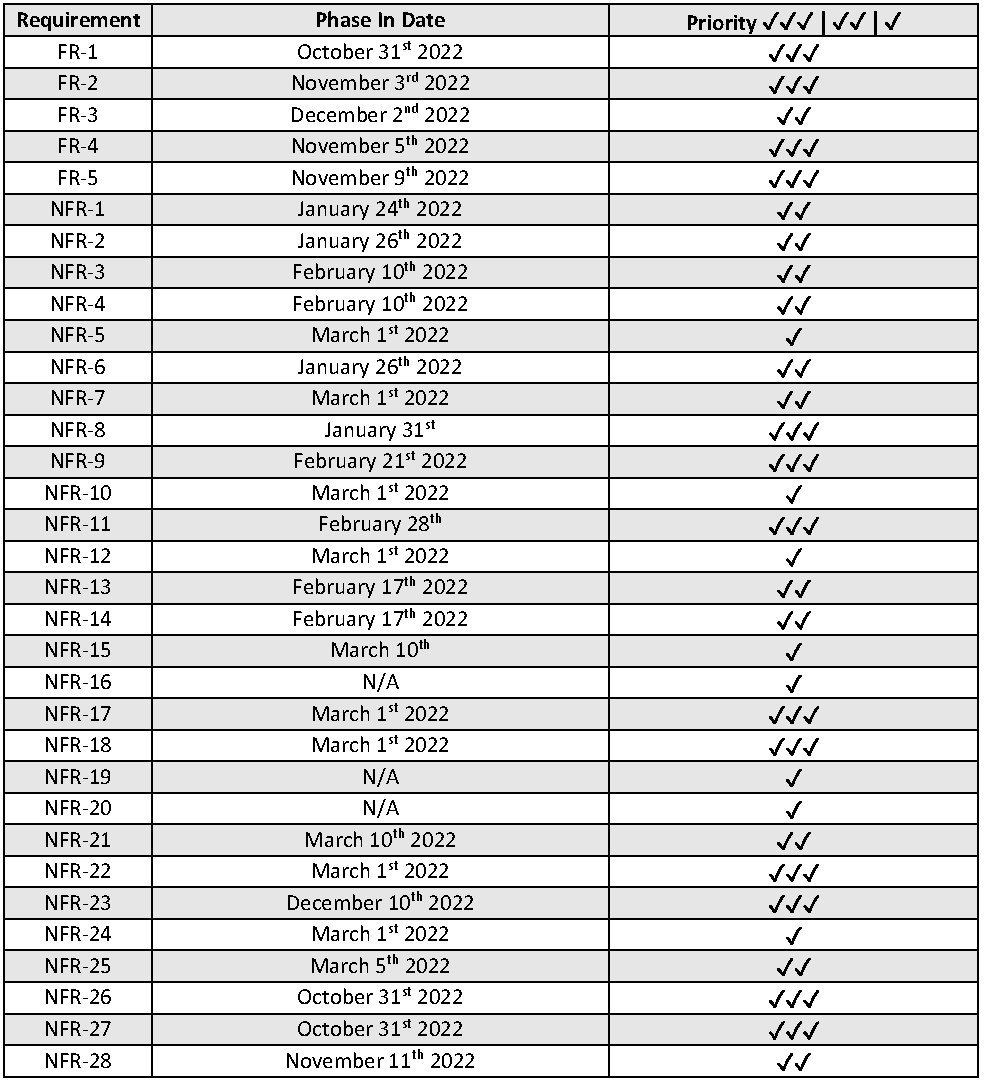
\includegraphics{P-diagram.pdf}
  \caption{Phase in Diagram}
  \label{PhaseDiagram} 
  \end{center}
\end{figure}

\noindent
The number of check marks within the Priority column in Figure \ref{PhaseDiagram} corresponds to the level of priority. Three check marks has a higher priority than two, and two check marks has a higher priority than one check mark.


\section{Project Issues}

\subsection{Requirements Likely/Unlikely to Change}
\begin{itemize}
  \item \textbf{FR} The functional requirements that were stated above are likely to remain the same as they are fundamental to the creation of the product. If any functional requirement happens to change, it would only be a slight deviation from the current requirements.
  \item \textbf{NFR-9} This non-functional requirement is likely to change as the processing time depends on the microcontroller we use. Ideally, we would use a high-speed microcontroller, however, cost and size are trade offs here. As a result, the processing times may change.
  \item \textbf{NFR-12} The battery life may vary according to the size and cost of the battery. Additionally, power consumption from the microcontroller will have to be considered when calculating the battery life. After further research into batteries and power consumption, will we be able to adjust this non-functional requirement to see if 12 hours of use is feasible.
  \item \textbf{NFR-14} this non-functional requirement may need to be adjusted to more or less keywords being \sout{able to detect} \textcolor{red}{detected}. This is dependent on the size of memory the microcontroller has.
  \item \textbf{NFR-21} this non-functional requirement may be changed to only interface with \sout{IOS} \textcolor{red}{Android} mobile devices as we have limited development time.
\end{itemize}

\subsection{Off-the-Shelf Solutions} 

\subsubsection{Ready-Made Products}
\label{readymade}
\begin{itemize}
  \item The Apple Watch contains a noise detection and alert function. The user can input specific sounds and the watch will notify the user if the noise is detected.
  \item The SoundWatch is another product which can detect sounds and notify the user when they are heard. The notifications come up on the watch to update users of heard sound.
  \item The Clarify wearable wristband, created by Neosensory, uses vibrations to notify users when a sound is detected.
\end{itemize}

\subsubsection{Reusable Components}
\begin{itemize}
  \item Small scale motors
  \item Speech recognition library, for example Google's Speech application programming interface
  \item CNN model trained on speech recognition (pretrained weights included) 
  \item Small scale microcontroller
  \item Small scale microphone
  \item Tutorial videos about how Java works, and how to improve user interface for application
  \item Gitlab, Github, Visual Studio Code are softwares that will help with creation and maintenance of code
\end{itemize}
\subsubsection{Products That Can Be Copied}
\begin{itemize}
  \item Certain aspects and features of ready-made products within section \nameref{readymade} will be considered as a guide to follow when developing the product.
\end{itemize}
\subsection{Tasks}

\subsubsection{Project Planning}

\begin{itemize}
  \item The Life Cycle will take on the V-Model
  \item Development approach will utilize CI/CD Pipeline
\end{itemize}

\subsubsection{Planning of the Development Phases}

\begin{figure}[H]
  \begin{center}
   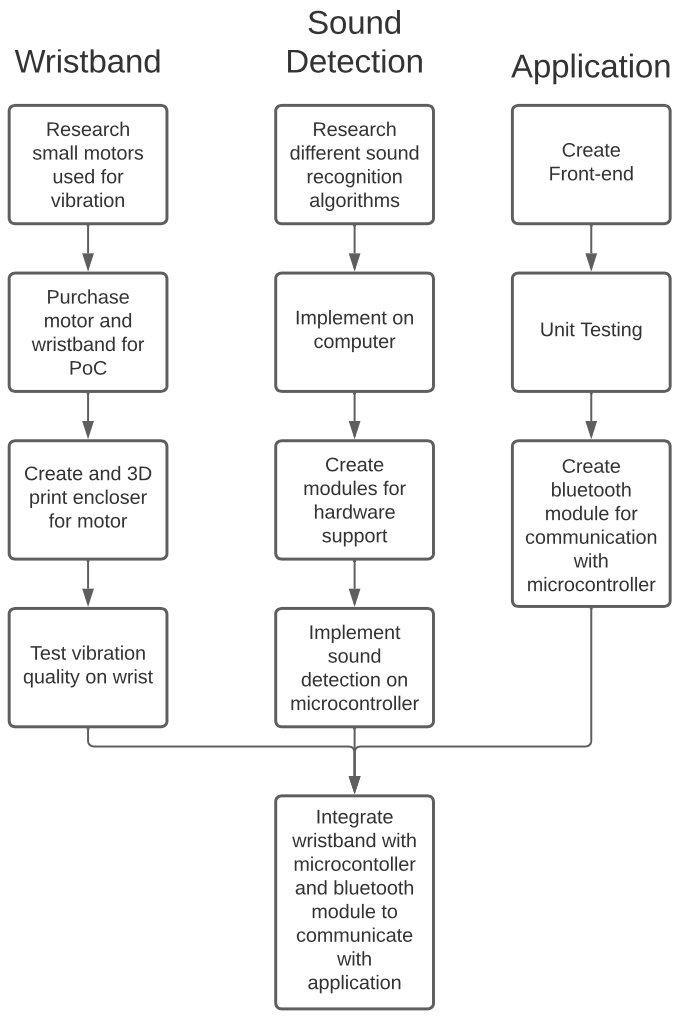
\includegraphics[width=0.5\textwidth, scale=0.5]{planning_dev_process.png}
  \caption{Tasks Diagram}
  \label{taskDiagram} 
  \end{center}
  \end{figure}

\subsection{Costs}
Highlighted below are the cost estimates for the project's physical system. Avoidable costs are the environmental set up and software, this is due to universal resource availability.
\center

\begin{tabular}{ |p{6cm}||p{3cm}| }
 \hline
 \multicolumn{2}{|c|}{Project Cost} \\
 \hline
 Description & Cost (in Canadian Dollars) \\
 \hline
FLORA Arduino Microcontroller   &  14.95    \\
 \hline
SparkFun Analog MEMS Microphone &   6.95  \\
\hline
Tatoko DC Motor &   25.04  \\
\hline
Silicone Watch Strap &   15.50  \\
\hline
5V Battery &   20.20  \\
\hline
Memory Card Reader &  6.94 \\
\hline

\end{tabular}
\captionof{table}{Project Cost}

\raggedright

\subsection{User Documentation and Training}

Documentation of the features and user application of the product will be provided in written and video format enabled with a unique QR code, which will be provided in packaging of the product.
Required training of the product will be needed to record initial sound detection. This is provided in the same user documentation used in the set-up stages.

\subsection{Risks}

\begin{itemize}
  \item Inaccurate sound detection - retrain that particular sound \textcolor{red}{with more training samples} to increase accuracy of product
  \item Wrong vibration pulse - reselect how many pulses required for particular sound
  \item Incorrect application signals - reboot device and user application to re sync user settings
\end{itemize}

\subsection{Future Developments}

Future developments will be conducted in different versions, listed below are the corresponding order from version 1.0 - version 4.0.

\begin{itemize}
  \item Double the microphones for improved sound detection
  \item Controlled vibration sensitivity through user application
  \item User LED display
  \item Compact design to fit in a wearable ring or necklace
\end{itemize}

\pagebreak

\section*{References}
\begin{itemize}
  \item https://www11.informatik.uni-erlangen.de/Lehre/WS1718/SW-SYS3/SWE-in-der-Praxis-WINF/volere-template.pdf
\end{itemize}

\section*{Reflection Appendix}
This section deals with what knowledge and experiences each team member will need 
to acquire so that the capstone project can be completed successfully. With that in 
mind, before identifying what each member is going to learn/master, some approaches 
of learning need to be established. Firstly, we believe that one of our main approaches 
to learning/mastering new skills is by scouring the internet for resources, videos, websites, 
blogs, or any other notable sources for relevant information. Another approach would be to 
look through books at McMaster's library to see if there is any applicable details that could 
be used for this project. Furthermore, one could also master their new skills via practice 
and trial-and-error by following tutorials and then trying to do them in real-time. Lastly, a 
final approach could be to find someone with relevant expertise and ask them for advice or 
some lessons on relevant skills/knowledge that would be beneficial for the project as a whole.

\subsection*{Jordan Bierbrier}
The knowledge that Jordan needs to acquire during this project is signal processing within a microcontroller. This is a crucial step for the project because we need to filter the incoming noise and extract meaningful information from the sound. This knowledge is important for the future as many products and technologies include signal processing. In order to learn more about signal processing, Jordan will talk to experts within the field to learn more about the techniques that are implemented. For example, past professors have a wealth of knowledge and there is a lot they can teach. Meetings will have to be scheduled with professors to learn more about the topics. Additionally, reviewing their course content would also help enrich Jordan’s knowledge of signal processing.   \\

\subsection*{Azriel Gingoyon}
The knowledge that Azriel needs to acquire for this project will be that of electrical 
circuitry and mechanical design. This is because he needs to be able to understand and 
learn of feasible, efficient, and effective ways to design the bracelet so that it can 
incorporate all of the necessary hardware for overall functionality while being non-intrusive 
for the user's comfortability. In terms of skills, it is most likely that he will need to 
become more proficient in CAD design, PCB design, circuit diagrams, and component research for 
cost-effective hardware to be used in the project.
\newline

\noindent
In regards to approaches to acquiring said knowledge or mastering these skills, Azriel believes
that the approach he should use is to scour the internet to learn more relevant information as 
well as do tutorials to improve applicable skills. This is because it is very effective to learn 
about new things from the web and its large databases of information. Furthermore, mastering skills 
can only be done through repetition and practice while continuously trying to learn new tricks/skills 
along the way.

\subsection*{Taranjit Lotey}
Knowledge of object-orientated programming for application development \\
Will be utilizing the web to master skills needed to have a deployable application.
Main focus will be on retaining information on certain functions and header files 
needed to create a user interface. Proxy communication will be required to communicate 
between the backend embedded system and frontend application.\\

\subsection*{Udeep Shah}
One of my approaches would be to learn from the web through articles and research documents. The other is to learn from my teammates.
For signal processing and filtering I would learn from research documents and web articles as these are more comprehensive and have a lot of detail for easy understanding of topics. For the writing aspect I would learn from my teammates as many of them have had to write requirements and technical documentation (software) that I have not done before. I select this approach as simply looking up on the web makes it a little too complicated in this case.


\subsection*{Abraham Taha}
The knowledge that Abraham needs to acquire for this project will include signal processing, mobile application development and speech recognition algorithms. Being the only software engineering student on the team these skills will be essential to creating the Front-end software portion of the project. Furthermore, improving knowledge in speech recognition will be essential for the core requirement of capturing keywords out of a data stream of sounds. More specifically, working with the programming languages of Swift and Java as they pertain to developing mobile applications will also be a key part of creating the final product. 
\newline

\noindent
These skills will be acquired through numerous avenues. First off, Youtube tutorials will be the main method. Youtube has a vast amount of resources for differing knowledge levels. Other avenues will include forum sites such as StackOverflow, these types of websites are useful for debugging programs through community help. Finally, another methodology for learning these skills will come from taking advantage of the opportunities at McMaster. Speaking with different professors who have experience in these issues will be great resources as we complete this project.

\end{document}